% Chapter 2

\chapter{The Application} % Main chapter title

\label{Chapter2} % For referencing the chapter elsewhere, use \ref{Chapter1} 

%----------------------------------------------------------------------------------------

% Define some commands to keep the formatting separated from the content 
%\newcommand{\keyword}[1]{\textbf{#1}}
%\newcommand{\tabhead}[1]{\textbf{#1}}
%\newcommand{\code}[1]{\texttt{#1}}
%\newcommand{\file}[1]{\texttt{\bfseries#1}}
%\newcommand{\option}[1]{\texttt{\itshape#1}}

%----------------------------------------------------------------------------------------

\section{Overview}
\paragraph In this chapter the application under test is described at high level and should be considered an introduction to \ref{Chapter3} where the application is described in greater detail but from the BDD point of view. As the development does not start from scratch but from a micro service Sprint demo, this chapter also describes what is already done and the improvements to be done during Project development based on BDD.

\paragraph The application consists on 6 services simulating an e-commerce application. A block diagram representation of the whole system is represented in figure \ref{fig:Block Diagram}.

\begin{figure}
\centering
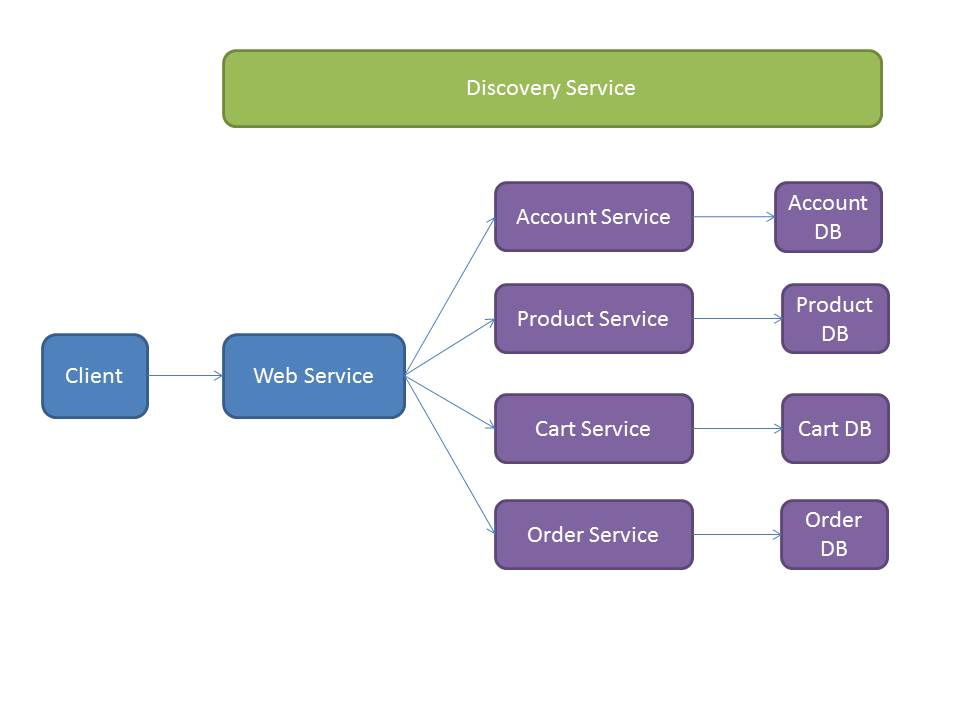
\includegraphics[width=\textwidth,height=\textheight,keepaspectratio]{Figures/Presentation1}
\decoRule
\caption[Block Diagram]{Application block diagram}
\label{fig:Block Diagram}
\end{figure}

\paragraph The user entry point is the Web Service, from where all the functionality of the application can be accessed. For the sake of simplicity there are no roles defined within the users of the application and thus any request coming from the Web Service is processed by the application.
There is no stock data either, considering that there is an unlimited amount available of each product added to the catalog represented by the Product Service database.
The Discovery Service is not focused on functional requirements but it tracks all the available instances of each running service.

\paragraph What follows is a short description of each one of the services:
\begin{itemize}
\item Web Service: User entry point. Application's functionality is accessed by the user through a UI provided by this service.
\item Account Service: Service for managing user accounts. Accounts can be created and deleted.
\item Product Service: Service that manages the shop product catalog. Products can be created and deleted.
\item Cart Service: Service that manages the products within the shopping carts.
\item Order Service: Service that manages the carts within the shopping orders.
\item Discovery Service: Service that manages the open instances of each one of the other services.
\end{itemize}

\paragraph Each one of the service implements and maintains its own relational database, without any link with other service's databases. Those services that need information from other services get it from the user through the Web Service. This means that the REST API exposed by all services consists at least on both "get" and "set" requests in order to be able to pull and push information from and to the system.
 
\paragraph Application behavior is shaped with the Gherkin files written for testing the services trying to simulate a BDD approach. More details on this follow in the next chapter. 

%----------------------------------------------------------------------------------------

\section{Data Model}

The Accounts, Product, Cart and Order Services have each one its own data model:\\


\textbf{Account Service}
\begin{itemize}
\item Number: int
\item Owner: string
\item Balance: float\\
\end{itemize}


\textbf{Product Service}
\begin{itemize}
\item Reference: string
\item Price: float
\item Description: string\\
\end{itemize}


\textbf{Cart Service}
\begin{itemize}
\item Name: string
\item AssociatedAccount: Account
\item AssociatedProducts: Product[]\\
\end{itemize}


\textbf{Order Service}
\begin{itemize}
\item Id: string
\item AssociatedCart: Cart\\
\end{itemize}

%----------------------------------------------------------------------------------------

\section{Technological Stack}
This application makes use of the following third party, open source libraries:

\begin{itemize}
\item Programming language: Java JDK v1.8: interoperability
\item Build tool: Apache Maven 3.3.9: defacto standard
\item Spring Framework Brixton Release: Spring Boot, Spring Cloud, Spring Data: project objective
\item Data Base: HyperSQL: integration with SPring
\item Test execution FW: JUnit 4.11: integration with Cucumber
\item Gherkin interpreter: cucumber-java 1.1.8: project objective
\item Docker Engine: 1.12.6: project objective
\end{itemize}


\section{Configuration}
The application is packaged within a single JAR file with all the services and the test framework with the Cucumber libraries and the implementation of the test steps for test execution. Having developed all services in one single project and thus using one single package certainly does not follow the philosophy of using micro services as it makes This simplifies showing how the application works. Each one of the services exposes a different port

\begin{itemize}
\item Web Service: 				localhost:1111
\item Account Service: 		localhost:2222
\item Product Service: 		localhost:3333
\item Order Service: 			localhost:4444
\item Cart Service: 			localhost:5555
\item Discovery Service: 	localhost:6666
\end{itemize}

All services are accessed thorugh one single Main class that will trigger one or other service depending on the arguments passed. So, the usage of the generated JAR file is the following:

\begin{itemize}
	\item java -jar sqa-project.jar [service]; where service is [accounts|products|carts|orders|web|registration]
\end{itemize}


\section{Assumptions}
\paragraph Some assumptions and restrictions have been done when programming the application mainly to ease the coding part of the application, which actually is not a topic included in the course agenda.\\
 
\begin{itemize}
\item There are no user roles within the application. Any user can both create products and accounts as well as create carts and buy products through orders. This might make no sense from the functional point of view but eases the programming of the application.\\

\item No stock data is used. Offering the possibility of increase and decrease the product stocks would create some relationships between services and their databases that would have added complexity to the coding.\\

\item All databases are initialized with one test entry:

\begin{itemize}
\item Account: 000000001, "TestUser", 1000
\item Product: ref001, "10", "Simple mouse"
\item Cart: C001, 000000001, ref001
\item Order: O001, C001
\end{itemize}
\end{itemize}